We use the CNN described in \citep{zhang2015character}.
The implementation is based on Torch \citep{torch} and available online\footnote{\url{https://github.com/zhangxiangxiao/Crepe}}.
In this section, we describe their design and the modifications we experimented with.
\subsection{Input}
\label{sub:input}
We first need to encode documents to a fixed sized sequence of vectors, so it can be fed to the temporal convolutional module described in Section \ref{sec:background}.
\cite{zhang2015character} do this by lowercasing the document, and mapping each character to a one-hot vector.
The alphabet used in our experiment is the same as in \citep{zhang2015character} and is 
\begin{verbatim}
abcdefghijklmnopqrstuvwxyz
0123456789
-,;.!?:’"/\|_@#$%ˆ&*˜‘+-=<>()[]{}
\end{verbatim} 
As the alphabet consists of 70 characters, each document is transformed into a sequence of vectors of size 70.
If a character in a document is not present in the alphabet, it is encoded to an all-zero vector.
Note that a whitespace is not part of the alphabet and therefore is also encoded to an all-zero vector.

\cite{zhang2015character} perform a data augmentation in order to avoid the generalisation error.
Specifically, they use an English thesaurus which is based on WordNet \cite{fellbaum1998wordnet} and replace words in the document to create a ``new'' example.
The number of words to be replaced and the index of the synonym used is chosen probabilistically.
This data augmentation technique is appropriate if the task is to classify the documents according to its semantics.
Indeed, the text classification tasks that \cite{zhang2015character} use this CNN for are sentiment analysis and topic classification.
Though the dataset we have is small and a data augmentation would have been useful, it was expected that this particular technique would introduce an undesirable noise in training for author profiling, as word choice is a crucial cue for the attributes of the author, especially their L1.
\cite{yarowsky2013learning} shows that the frequency distribution of words used in a corpus of computational linguistics articles from the ACL Anthology varies greatly from L1 to L1 of the author.
For instance, a word ``claim'' is much less often used by Chinese native speakers than native speakers of other languages, and ``complementary'' is more frequently used by French or Spanish native speakers.
The latter can potentially be explained by the latin origin of the word.
To preserve such distinguishing features in the data, we turned off the data augmentation.

In \citep{zhang2015character}, the first 1014 characters are taken from each document and encoded to be used as an input.
This is potentially problematic with the dataset we have.
As shown in Table \ref{tab:tr-stat}, majority of the documents in the training set is significantly shorter than 1014 characters.
Though pooling should help the model to be invariant to the location of a feature, having majority of the training examples padded extensively might be harmful.

To partially mitigate the problem of small dataset and short documents, during the training, instead of feeding the first 1014 characters of the document to the model, we take a window of smaller size at an arbitrary location.
For instance, given a document of length 1000 and a window size $l_w = 100$, a CNN may sample 100 characters at 900 different locations, effectively creating 900 different examples.
In this report, we refer to this approach as \emph{random window sampling}.
For testing, we take the window of the same size at the beginning of the document for an easier comparison of the results.

We experiment with $l_w \in \{123, 339, 555, 771, 1014\}$.
Note that these numbers are chosen as they are compatible with the architecture.
\subsection{Architecture}
\begin{figure*}[h]
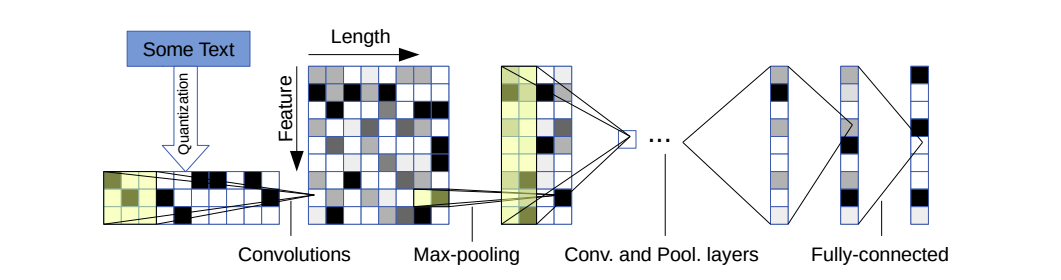
\includegraphics[width=\textwidth]{architecture.png}
\caption{Overview of Architecture}
\label{fig:architecture}
\end{figure*}

Figure \ref{fig:architecture} gives an illustration of the model described in \citep{zhang2015character}, which we use without modification.
The CNN consists of 6 convolutional, and 3 fully-connected layers.
The kernel described in Section \ref{sub:conv} is applied with stride 1.
The activation function used is a threshold function $th$ defined as follows:
\[
  th(x) =
  \begin{cases}
    x & \text{if $x > 1\mathrm{e}{-6}$} \\
    0 & \text{otherwise}
  \end{cases}
\]
Max-pooling is applied with stride 3 at first, second and sixth convolutional layer.
Table \ref{tab:conv-config} shows the configuration of the convolutional layers.
\begin{table*}[t]
\centering
\caption{Convolutional Layers Used in \citep{zhang2015character}}
\label{tab:conv-config}
\begin{tabular}{cccc}
Layer & Frame Size & Kernel Width & Pooling Region Width \\ \hline
1     & 256        & 7            & 3                    \\
2     & 256        & 7            & 3                    \\
3     & 256        & 3            & N/A                  \\
4     & 256        & 3            & N/A                  \\
5     & 256        & 3            & N/A                  \\
6     & 256        & 3            & 3                   
\end{tabular}
\end{table*}
The number of features of the input is 70, which is the size of the alphabet given in \ref{sub:input}.
As stated previously, in \citep{zhang2015character} the length of the input is 1014.
With our approach of random window sampling, the length of the input is equal to the window size $l_w$.
The output frame length after the last convolutional layer is $(l_0 - 96) / 27$, where $l_0$ is the length of the input.
This defines a set of possible window sizes $l_w$.

Between the fully-connected layers, dropout modules \citep{hinton2012improving} with dropout probability of 0.5 are used for regularisation.
Seventh and eighth layer have 1024 output units, and ninth layer have three as this is applied to three-class classification.

At each epoch, a minibatch of size 128, chosen randomly from the training set, is used to update the weight with stochastic gradient decent \citep{polyak1964some} with momentum \citep{sutskever2013importance} 0.9 and step size 0.01.
